
%%%%%%%%%%%%%%%%%%%%%%%%%%%%%%%%%%%%%
%%%%%%%%%%%%%%%%%%%%%%%%%%%%%%%%%%%%%
%
%   Hi, All
%   Arun Xavier, VAST Thrissur
%
%   for more  Visit my Page - http://arunxeee.blogspot.in/
%
%%%%%%%%%%%%%%%%%%%%%%%%%%%%%%%%%%%%
%%%%%%%%%%%%%%%%%%%%%%%%%%%%%%%%%%%%
%%%%%%%%%%%%%%%%%%%%%%%%%%%%%%%%%%%%%
%%%%%%%%%%%%%%%%%%%%%%%%%%%%%%%%%%%%%
%
%   Hi, All
%   Arun Xavier, VAST Thrissur
%
%   for more  Visit my Page - http://arunxeee.blogspot.in/
%
%%%%%%%%%%%%%%%%%%%%%%%%%%%%%%%%%%%%
%%%%%%%%%%%%%%%%%%%%%%%%%%%%%%%%%%%%

%%
\documentclass[12 pt, oneside]{book}
\usepackage{graphicx, fancyhdr, amsmath, times, enumerate,geometry,makeidx,setspace,nomencl,eso-pic,xcolor,lipsum,calc,pst-node,tikz,fancybox,background,caption,subcaption,amsfonts}




\usetikzlibrary{calc}
\SetBgScale{1}
\SetBgAngle{0}
\SetBgColor{brown}
\SetBgOpacity{1}
%%
\geometry{verbose,a4paper,tmargin=1 in,bmargin=1in,lmargin=1.5 in,rmargin=.9 in}
%%%%%%%%%%%%%%%%%%%%%%%%%%%%%%%

\makeindex

%%
\usepackage[final]{pdfpages}
%%
%\setlength{\oddsidemargin}{2 cm}



%%
\newcommand{\VAtitle}[1]%
{\def\vtitle{#1}}%
\newcommand{\VAauthora}[1]%
{\def\vauthora{#1}}%
\newcommand{\VAauthorb}[1]%
{\def\vauthorb{#1}}%
\newcommand{\VAauthorc}[1]%
{\def\vauthorc{#1}}%
\newcommand{\VAauthord}[1]%
{\def\vauthord{#1}}%
\newcommand{\VAauthore}[1]%
{\def\vauthore{#1}}%
\newcommand{\VAadmissionyear}[1]%
{\def\vadmissionyear{#1}}%
\newcommand{\VAacademicyear}[1]%
{\def\vacademicyear{#1}}%
\newcommand{\VAprincipal}[1]%
{\def\vprincipal{#1}}%
\newcommand{\VAguide}[1]%
{\def\vguide{#1}}%
\newcommand{\VAguidedg}[1]%
{\def\vguidedg{#1}}%
\newcommand{\VAhod}[1]%
{\def\vhod{#1}}%
\newcommand{\VAdate}[1]%
{\def\vdate{#1}}%
\newcommand{\VAdept}[1]%
{\def\vdept{#1}}%
\newcommand{\VAclass}[1]%
{\def\vclass{#1}}%
\newcommand{\VApaper}[1]%
{\def\vpaper{#1}}%
%%
%%



\SetBgContents{}



\VApaper{MAIN PROJECT REPORT}

\usepackage{titlesec}
\titleformat{\chapter}[display]
{\normalfont\LARGE\bfseries\centering}{\chaptertitlename\ \thechapter}{20pt}{\Huge}

\begin{document}
%%%%%%%%%%%%%%%%%%%%%%%%%%%%%%%%%%%%
%%%%%%%%%%%%%%%%%%%%%%%%%%%%%%%%%%%%
%%
%%          Edit the Names & others from below onwards. . .
%%
%%%%%%%%%%%%%%%%%%%%%%%%%%%%%%%%%%%%
%%%%%%%%%%%%%%%%%%%%%%%%%%%%%%%%%%%%

\VAtitle{DETECTION AND PREDICTION OF AIR POLLUTION LEVEL}

%%%%%%%%%%%%%%%%%%%%%%%%%%%%%%
%   
%	Give Students name in Alphabetical Order 
%
%%%%%%%%%%%%%%%%%%%%%%%%%%%%%%
\VAauthora{SRUTHI K S}
\VAauthorb{TESLIN ROSE P V}
\VAauthorc{VINI SASIDHARAN}
\VAauthord{VISHNU V U}

%%%%%%%%%%%%%%%%%%%%%%%%%%%%%%%%
%
%	Give details of Main Author, (to be seen in the certificate, etc.)
%
%%%%%%%%%%%%%%%%%%%%%%%%%%%%%%%%
%
\VAadmissionyear{2016}
%
%%%%%%%%%%%%%%%%%%%%%%%%%%%%%%%%
\VAprincipal{Dr. Saji C.B}
\VAguide{Ms. Nitha K P}
\VAguidedg{Asst. Prof.,}  % Give your Guides Designation Asst. Prof., Asso. Prof.
\VAhod{Dr. Ramani Bai V }
\VAdate{November 2019}
\VAacademicyear{2019-2020}%
\VAdept{Computer Science and Engineering}
\VAclass{B.Tech (CSE)}

%%%%%%%%%%%%%%%%%%%%%%%%%%%%%%%%%%%%
%%%%%%%%%%%%%%%%%%%%%%%%%%%%%%%%%%%%

\pagestyle{empty}
%%%%%%%%%%%%%%%%%%%%%%%%%%%%%%%%%%%%%
%%%%%%%%%%%%%%%%%%%%%%%%%%%%%%%%%%%%%
%
%   Hi, All
%   Arun Xavier, VAST Thrissur
%
%   for more  Visit my Page - http://arunxeee.blogspot.in/
%
%%%%%%%%%%%%%%%%%%%%%%%%%%%%%%%%%%%%
%%%%%%%%%%%%%%%%%%%%%%%%%%%%%%%%%%%%
%
%******************************************************
%

\begin{spacing}{1.5}
\begin{titlepage}




\SetBgContents{

\begin{tikzpicture}[overlay,remember picture]
\draw [line width=3pt]
    ($ (current page.north west) + (3.0cm,-1.8cm) $)
    rectangle
    ($ (current page.south east) + (-1.35cm,1.8cm) $);
\draw [line width=1pt]
    ($ (current page.north west) + (3.15cm,-1.95cm) $)
    rectangle
    ($ (current page.south east) + (-1.5cm,1.95cm) $); 
\end{tikzpicture}
}

\begin{center}


{ \LARGE \rmfamily \bf \vtitle}\\[1 cm]

{ \large \rmfamily A \vpaper \\ SUBMITTED IN PARTIAL FULFILLMENT OF THE \\REQUIREMENTS FOR THE AWARD OF DEGREE OF}\\[1 cm]

{ \Large \rmfamily \bf BACHELOR OF TECHNOLOGY}\\
{\large \rmfamily in}\\[.2 cm]
{ \Large \rmfamily \bf COMPUTER SCIENCE AND ENGINEERING}\\
{\large \rmfamily of}\\[.2 cm]
{ \Large \rmfamily \bf APJ Abdul Kalam Technological University}\\
{\large \rmfamily by}\\[.2 cm]
{\large \rmfamily \bf \vauthora } \\
{\large \rmfamily \bf \vauthorb } \\
{\large \rmfamily \bf \vauthorc } \\
{\large \rmfamily \bf \vauthord } \\[1.5 cm]
%{\large \rmfamily \bf \vauthore } \\
%

%
\includegraphics[width=3.5 cm]%
{VidyaLogo.JPG}\\
\scriptsize (AN ISO 9001:2008 CERTIFIED INSTITUTION )\\[.4 cm]


%
{\Large \bf Department of \vdept}\\
{\Large \rmfamily Vidya Academy of Science \& Technology\\[.2 cm]
\large Thalakkottukara, Thrissur - 680 501}\\
({ \bf \tt http://www.vidyaacademy.ac.in})\\[.4 cm]
{\large \rmfamily \vdate}


\end{center}
\end{titlepage}
%
%******************************************************
%
\clearpage


\pagenumbering{gobble}
%\pagestyle{empty}
\addcontentsline{toc}{chapter}{\quad CERTIFICATE}




\begin{titlepage}
\SetBgContents{

\begin{tikzpicture}[overlay,remember picture]
\draw [line width=3pt]
    ($ (current page.north west) + (3 cm,-1.8cm) $)
    rectangle
    ($ (current page.south east) + (-1.5cm,1.8cm) $);
\draw [line width=1pt]
    ($ (current page.north west) + (3.15cm,-1.95cm) $)
    rectangle
    ($ (current page.south east) + (-1.65cm,1.95cm) $); 
\end{tikzpicture}
}


\begin{center}


{\Large \bf Department of \vdept  }\\
{\Large \bf Vidya Academy of Science \& Technology}\\
{\normalsize \bf Thalakkottukara, Thrissur - 680 501\\
({\tt http://www.vidyaacademy.ac.in})}\\[0.75cm]
%
%   Logo
%

\includegraphics[width=3.5 cm]{VidyaLogo.JPG}\\
\scriptsize (AN ISO 9001:2008 CERTIFIED INSTITUTION )\\[.3 cm]
%
 \Huge  $ \mathfrak{Certificate}$\\[0.3cm]
%
\end{center}
\index{Certificate}
\index{University of Calicut}

\quad This is to certify that the Main Project Report titled {\bf ``\vtitle"} is a bonafide record of the work carried out by {\bf \vauthora\ ,\vauthorb\ ,\vauthorc\ ,\vauthord\ }  of Vidya Academy of Science \& Technology, Thalakkottukara, Thrissur - 680 501 in partial fulfillment of the requirements for the award of  {\bf Degree of Bachelor of Technology} in {\bf Computer Science and Engineering} of  {\bf APJ Abdul Kalam Technological University}, during the academic year \vacademicyear. The Main Project report has been approved as it satisfies the academic requirements in the respect of main project work prescribed for the said degree.\\[.3cm]
 
\noindent{\bf Project Guide/Supervisor} \hfill  {\bf Project Coordinator} \\[.3cm]
\noindent \vguide \hfill .................................\\  Prof.,Dept. of CSE  \\.................. \\   \hfill  \\\hspace*{\fill} {\bf Head of Department}\noindent  \\\hspace*{\fill} \hfill\vhod  \\\hspace*{\fill}\hfill  Prof.,Dept. of CSE \\\hspace*{\fill}
\hfill .................................\\ 



%
\end{titlepage}

%   End of Certificate
%  
\clearpage

%\pagestyle{empty}
\addcontentsline{toc}{chapter}{\quad UNDERTAKING}
%%%%%%%%%%%%%%%%%%%%%%%%%%%%%%%%%%%%%
%%%%%%%%%%%%%%%%%%%%%%%%%%%%%%%%%%%%%
%
%   Hi, All
%   Arun Xavier, VAST Thrissur
%
%   for more  Visit my Page - http://arunxeee.blogspot.in/
%
%%%%%%%%%%%%%%%%%%%%%%%%%%%%%%%%%%%%
%%%%%%%%%%%%%%%%%%%%%%%%%%%%%%%%%%%%
%


\begin{titlepage}


\SetBgContents{

\begin{tikzpicture}[overlay,remember picture]
\draw [line width=3pt]
    ($ (current page.north west) + (3.0cm,-1.8cm) $)
    rectangle
    ($ (current page.south east) + (-1.5cm,1.8cm) $);
\draw [line width=1pt]
    ($ (current page.north west) + (3.15cm,-1.95cm) $)
    rectangle
    ($ (current page.south east) + (-1.65cm,1.95cm) $); 
\end{tikzpicture}
}

\chapter*{\centering Undertaking}
%


\quad \quad We, {\bf \vauthora , \vauthorb , \vauthorc , \vauthord  }, hereby undertake that, the main project work entitled {\bf ``\vtitle"}, is carried out by us independently under the valuable guidance of {\bf \vguide}, \vguidedg\ Dept. of \vdept, Vidya Academy of Science and Technology, Thalakkottukara, Thrissur, in partial fulfillment of the requirements for the award of degree of {\bf Bachelor of Technology in Computer Science Engineering } of APJ Abdul Kalam Technological University, during the academic year \vacademicyear.\\[1 cm]

\begin{flushright}
{\bf \vauthora(VAS16CS116)\\
\vauthorb(VAS16CS119)\\
\vauthorc(VAS16CS123)\\
\vauthord(LVAS16CS136)\\	
}
\end{flushright}
\noindent Thrissur \\
\vdate 


\end{titlepage}




\clearpage



%   Redefining plain page style
%  
\fancypagestyle{plain}{%
\fancyhf{} % clear all header and footer fields
\fancyhead[L]{{\scriptsize \vtitle}}
\fancyhead[R]{
\includegraphics[width=0.5cm]{VidyaLogo.JPG}}
%\fancyfoot[C]{\bfseries \thepage} 
\fancyfoot[L]{{\footnotesize Department of Computer Science Engg.}}
\fancyfoot[R]{\footnotesize VAST, Thalakotukara}
\fancyfoot[C]{\footnotesize \bf \thepage}%
\renewcommand{\headrulewidth}{1pt}%
\renewcommand{\footrulewidth}{1pt}%
}%
%

\pagenumbering{roman}

\pagestyle{plain}
\addcontentsline{toc}{chapter}{\quad ACKNOWLEDGEMENT}
%%%%%%%%%%%%%%%%%%%%%%%%%%%%%%%%%%%%%
%%%%%%%%%%%%%%%%%%%%%%%%%%%%%%%%%%%%%
%
%   Hi, All
%   Arun Xavier, VAST Thrissur
%
%   for more  Visit my Page - http://arunxeee.blogspot.in/
%
%%%%%%%%%%%%%%%%%%%%%%%%%%%%%%%%%%%%
%%%%%%%%%%%%%%%%%%%%%%%%%%%%%%%%%%%%


%
\chapter*{\centering Acknowledgement}
%


\par
\hspace{0.9cm}During the course of our main project work several persons collaborated directly and indirectly with us. Without their support it would be impossible for us to finish our work. That is why we wish to dedicate this section to recognize their support.
\vspace {.2cm}
\par
\hspace{.35cm}We want to start expressing our thanks to our project guide {\bf \vguide}, \vguidedg\ Dept. of \vdept, because of his valuable advice and guidance towards this work. We received motivation, encouragement and hold up from his during the course of work.

\vspace{0.2cm}
\par
\hspace{0.35cm}We are grateful to express our thanks to all the faculty members of our department for their support. We articulate our gratitude to all my friends for their support and help for this work.

\vspace{.2cm}
\par 
\hspace{.35cm}We thankful to {\bf \vhod}, 
Head of \vdept\  Department, and our Principal {\bf \vprincipal}, for their sole co-operation.

\vspace{0.2cm}
\par
\hspace{0.35cm}Last, but not the least we wish to express our gratitude to God Almighty for His abundant blessings without which this effort would not have been successful.\\[.3 cm]



\begin{flushright}
{\vauthora , \vauthorb , \vauthorc , \vauthord }

\vclass\  (\vadmissionyear\  Admissions)\\
Vidya Academy of Science \& Technology\\
\vdate  \hfill Thrissur - 680 501.
\end{flushright}






%%%%%%%%%%%%%%%%%%%%%%%%%%%%%%%%%%%%
%%%%%%%%%%%%%%%%%%%%%%%%%%%%%%%%%%%%

\chapter*{\centering{Abstract}}
\addcontentsline{toc}{chapter}{\quad ABSTRACT}

Air pollution has become an important public health concern The high concentration of fine particulate matter with diameter less than 2.5 $\mu$m (PM 2.5 ) is known to be associated with lung cancer, cardiovascular disease, respiratory disease, and metabolicdisease.
Predicting Air Quality can help governments warn people at high risk, thus mitigating the complications. 
\par In this work feature importance of air pollution, Implementing Random forest, XGBoost, CatBoost and Deep learning machine learning (ML) approaches.
We use 8 features, including meteorological data, ground-measured PM 2.5 and gaseous pollutants. forecasting Air quality using deep learning technique LSTM and Prophet package by Facebook we can extract the trend yearly seasonality, and weekly seasonality of the time series 

%%%%%%%%%%%%%%%%%%%%%%%%%%%%%%%%%%%%
%%%%%%%%%%%%%%%%%%%%%%%%%%%%%%%%%%%%
%       
%		Do not change any thing after this . . .
%
%%%%%%%%%%%%%%%%%%%%%%%%%%%%%%%%%%%%
%%%%%%%%%%%%%%%%%%%%%%%%%%%%%%%%%%%%
\tableofcontents
\addcontentsline{toc}{chapter}{\quad  LIST OF FIGURES}
\listoffigures
% For adding List of symbols or abbreviations
\mainmatter
%%%%%%%%%%%%%%%%%%%%%%%%%%%%%%%%%%%%%
%%%%%%%%%%%%%%%%%%%%%%%%%%%%%%%%%%%%%
%%    
%%    Copy your Project Work below from Here
%%
%%%%%%%%%%%%%%%%%%%%%%%%%%%%%%%%%%%%%
%%%%%%%%%%%%%%%%%%%%%%%%%%%%%%%%%%%%%


\chapter {INTRODUCTION}
	
\section{General}    % For giving Section  eg: 1.1
As a consequence of urbanization and
industrialization, air pollution has become one of
the most important public health concerns. The
PM 2.5 pollutant is defined as fine inhalable
particles with diameters less than 2.5 $\mu$m. The
association of high PM 2.5 concentration and
cancer, cardiovascular disease, respiratory
disease, metabolic disease, and obesity has been
proven.
\par Particulate matter can be either
human-made or naturally occur.Some examplesinclude dust, ash and sea-spray. Particulate matter
(including soot) is emitted during the combustion
of solid and liquid fuels, such as for power
generation, domestic heating and in vehicle
engines. Particulate matter varies in size.
Different machine learning models have been
applied to detect air pollution and predict PM2.5
levels based on a data set consisting of daily
atmospheric conditions. Although several
attempts have been made to predict PM 2.5
concentration, the relationship between features
that influence PM 2.5 concentration prediction is
still not well understood.

% You can add any sections like that . . . 

\section{Objectives of the Work}
This system exploits machine learning models
to predict and forecast PM2.5 levels based on a
data set consisting of atmospheric conditions in a
specific city. \pagebreak \linebreak

The proposed system does two tasks
\begin{description}
  \item[$\bullet$ (i)]  predict the levels of PM2.5 based on given historical values.
  \item[$\bullet$ (ii)]   Forecast the level of PM2.5 for 7 days.
\end{description}
Random forest, Extreme gradient boost, CatBoost
and Deep learning are employed to predict the
level of PM 2.5 based on the previous readings.
The primary goal is to predict the air pollution
level in the City with the ground data set.
Prophet and LSTM is used to forecast the PM2.5 level upto 7 Days.


\section{Motivation for this work}

Considering the daily newspapers and any other electronic or print media, a devastating
news which is spreading day by day is people is becoming sick and the climate is changing such
a way that it has become miserable for living of people. From the aspect from top to bottom,
every people are suffering the curse of climate change. The main reason for the climate change
and people health is air pollution. It has brought changes in climate like global warming, global
dimming, over raining, drought, storms, acid rain, foggy weather etc. The living things on earth
and under water are suffering many problems like change in life due to lack of proper facilities
of life. 
Continued exposure to environments with poor air quality is a major public health concern in
developed and developing countries. It is estimated that the pollutants responsible for poor air
quality cause nearly 2.5 million premature deaths per year world-wide. Significantly, around 1.5
million of these deaths are due to polluted indoor air, and it is suggested that poor indoor air
quality may pose a significant health risk to more than half of the world’s population. Due to its
link with industrialisation, societal health problems associated with poor air quality
disproportionately affects developed and developing nations – it is estimated that air pollution is
responsible for the premature deaths. 
Air is the most useful thing for each and every living thing. Researching on this serious
issue this system’s main purpose was to estimate the quality of air for people and any other
living thing which exist on earth. Very important to know for our living is that how much safe
we are now and how the weather and climate has changed for air pollution and it will sustain
sound. \

\pagebreak
\section{Methodologies Adopted}
For the project, we evaluated several different types of prediction and forecast machine learning  models which will be described below. We use Prophet and LSTM for forecasting air quality and XGBoost,Random Forest, CatBoost and Deep Learning for prediction.Data processing and matching is necessary because the data is obtained from different sources.Therefore, we intend to use interpolation to estimate and fill in the missing data.Data normalization is an important step for many machine-learning estimators. A correlation matrix can be used to investigate the dependence between multiple variables at the same time


\section{Outline of the Report}
This report contains 4 chapters. Chapter 1 gives the introduction to the project work and
describes the objectives of the work. Literature survey is describes in Chapter 2. System
Design is explained in the chapter 3 and Methodology  is well explained
in chater 4. 


\chapter{LITERATURE REVIEW}

\section{A Machine Learning Approach for Air Quality Prediction: Model Regularization and Optimization}

Dixian Zhu ,Changjie Cai , Tianbao Yang and Xun Zhou 

In this paper, we tackle air quality forecasting by using machine learning approaches
to predict the hourly concentration of air pollutants (e.g., ozone, particle matter (PM2.5) and sulfur
dioxide). Machine learning, as one of the most popular techniques, is able to efficiently train a model
on big data by using large-scale optimization algorithms. Although there exist some works applying
machine learning to air quality prediction, most of the prior studies are restricted to several-year
data and simply train standard regression models (linear or nonlinear) to predict the hourly air
pollution concentration. In this work, we propose refined models to predict the hourly air pollution
concentration on the basis of meteorological data of previous days by formulating the prediction over
24 h as a multi-task learning (MTL) problem. This enables us to select a good model with different
regularization techniques. We propose a useful regularization by enforcing the prediction models of
consecutive hours to be close to each other and compare it with several typical regularizations for
MTL, including standard Frobenius norm regularization, nuclear norm regularization, and `2,1-norm
regularization. Our experiments have showed that the proposed parameter-reducing formulations
and consecutive-hour-related regularizations achieve better performance than existing standard
regression models and existing regularizations.

In this paper, we have developed efficient machine learning methods for air pollutant prediction.
We have formulated the problem as regularized MTL and employed advanced optimization algorithms
for solving different formulations. We have focused on alleviating model complexity by reducing the
number of model parameters and on improving the performance by using a structured regularizer.
Our results show that the proposed light formulation achieves much better performance than the
other two model formulations and that the regularization by enforcing prediction models for two
consecutive hours to be close can also boost the performance of predictions. We have also shown that
advanced optimization techniques are important for improving the convergence of optimization and
that they speed up the training process for big data. For future work, we will further consider the
commonalities between nearby meteorology stations and combine them in a MTL framework, which
may provide a further boosting for the prediction.

\section{A Deep Learning Approach for Forecasting Air Pollution in South Korea Using LSTM}

Tien-Cuong Bui, Van-Duc Le, Sang K. Cha

Over the last few years, tackling air pollution is an urgent problem in
South Korea. Much research is being conducted in environmental science to
evaluate the severe impact of particulate matters on public health. Besides that,
deterministic models of air pollutant behavior are also generated; however, these
are both complex and often inaccurate. On the contrary, deep recurrent neural
network reveals strong potential on forecasting outcomes of time-series data and
has become more prevalent. This paper uses Recurrent Neural Networks and
Long Short-Term Memory units as a framework for leveraging knowledge from
time-series data of air quality and meteorological information. Finally, we
investigate prediction accuracies of various configurations. This paper is a
significant motivation for not only continuing researching on urban air quality
but also helping the government leverage that insight to enact beneficial policies.

The goal of the presented work was to evaluate the effectiveness of encoder-decoder
networks for building prediction machines with time series data. The proposed model
shows significant results in prediction PM2.5 AQI of long future based on historical
meteorological data. However, to enhance the accuracy of the prediction machine, the
model needs to be evaluated more in the future. Finally, forecasting the status of air
pollution can help governments in policy-making and resource allocation.

\section{Prediction Model of Air Pollutant Levels Using Linear Model with Component Analysis}

Arie Dipareza Syafei, Akimasa Fujiwara, and Junyi Zhang

Abstract—The prediction of each of air pollutants as
dependent variable was investigated using lag-1(30 minutes
before) values of air pollutants (nitrogen dioxide, NO2,
particulate matter 10um, PM10, and ozone, O3) and
meteorological factors and temporal variables as independent
variables by taking into account serial error correlations in the
predicted concentration. Alternative variables selection based
on independent component analysis (ICA) and principal
component analysis (PCA) were used to obtain subsets of the
predictor variables to be imputed into the linear model. The
data was taken from five monitoring stations in Surabaya City,
Indonesia with data period between March-April 2002. The
regression with variables extracted from ICA was the worst
model for all pollutants NO2, PM10, and O3 as their residual
errors were highest compared with other models. The
prediction of one-step ahead 30-mins interval of each pollutant
NO2, PM10, and O3 was best obtained by employing original
variables combination of air pollutants and meteorological
factors. Besides the importance of pollutants interaction and
meteorological aspects into the prediction, the addition spatial
source such as wind direction from each monitoring station has
significant contribution to the prediction as the emission
sources are different for each station.

There is a concern of adverse effect to humans health due
to high concentration of pollutants which exceed the standard
value. These events occur often and people should get alerted
when this happens, thus making the short-term prediction of
pollutant become crucial. Linear models with original
variables, ICs, and PCs extracted from six pollutants (NO,
NO2, O3, SO2, CO, PM10 and meteorological factors (wind
speed, solar gradiation, humidity and temperatures) were
employed to predict 30-mins ahead of NO2, PM10, and O3. In
addition, we include serial error correlation computation in
the model for model accuracy. As expected, the presence of
NO has positive correlation with NO2, aside with CO, wind
speed and solar gradiation. Furthermore, it was shown that
meteorologica factors have high role in the formation of O3.
The faster wind speed will reduce the concentration of NO2
while on the opposite will increase the concentration of O3.
This pattern is also found for humidity. Since PM10 is
relatively inert particle gas with less than 10um, using the
30-mins data we obtained, no significant correlation was
found with other variables.

\section{Industrial Air Pollution Prediction Using Deep Neural Network}

Yu Pengfei, He Juanjuan, Liu Xiaoming, and Zhang Kai

In this paper, a deep neural network model is proposed to
predict industrial air pollution, such as PM2.5 and PM10. The deep
neural network model contains 9 hidden layers, each layer contains 45
neurons. The output of the hidden layer neurons is calculated using the
ReLU activation function, which can effectively reduce the gradient elim-
ination effect of the deep neural network. Twelve air pollutant indicators
from industrial factories are collected as the input data, such as CO,
NO2, O3, and SO2. About 180,000 real industrial air pollution data from
Wuhan City are used to train and test the DNN model. Furthermore,
the performance of our approach is compared with the SVM and Artifi-
cial neural network methods, and the comparison result shows that our
algorithm is accurate and competitive with higher prediction accuracy
and generalization ability.

In this paper, we proposed a deep neural network model to predict industrial
air pollutant. About 180,000 real industrial air pollution data from 2016 to 2018
in Wuhan are used to train, validate and test the model. We use ReLU non-
linear activation function instead of the traditional Sigmoid activation function,
effectively improve the training speed of the network, eliminating the gradient
disappearance or gradient explosion phenomenon. We use the Batch Normal-
ization method to improve the training accuracy and convergence speed of the
network. Through the DropOff technology, effectively prevent the depth of the
neural network over-fitting, improve the test data prediction accuracy. The per-
formance of our approach is compared with the SVM and BP neural network,
and the comparison result shows that our algorithm is accurate and competitive
with higher prediction accuracy and generalization ability.

\section{Air Pollution Forecasting Using a Deep Learning
Model Based on 1D Convnets
and Bidirectional GRU}

QING TAO, FANG LIU , (Member, IEEE), YONG LI , (Senior Member, IEEE), DENIS SIDOROV, (Senior Member, IEEE)

Air pollution forecasting can provide reliable information about the future pollution situation,
which is useful for an efficient operation of air pollution control and helps to plan for prevention. Dynamics
of air pollution are usually reflected by various factors, such as the temperature, humidity, wind direction,
wind speed, snowfall, rainfall, and so on, which increase the difficulty in understanding the change of air
pollutant concentration. In this paper, a short-term forecasting model based on deep learning is proposed for
PM2.5 concentration, and the
convolutional-based bidirectional gated recurrent unit (CBGRU) method is presented, which combines 1D
convnets (convolutional neural networks) and bidirectional GRU (gated recurrent unit) neural networks. The
case is carried out by using the Beijing PM2.5 data set in UCI Machine Learning Repository. Comparing the
prediction results with the traditional ones, it is proved that the error of the CBGRU model is lower and the
prediction performance is better.


The results are compared with traditional mechine learning
models and conventional deep learning models. The results
show that the proposed method can be suitable and compet-
itive on the PM2.5 data time series forecasting. To be more
specific, compared with shallow machine learning models,
such as DTR, SVR and GBR, deep learning-based methods
exhibited better prediction performance. Furthermore, com-
pared with GRU, bidirectional GRU has lower error value,
which indicates that the use of bidirectional GRU can improve
the prediction effect. This is because the bidirectional GRU
processes the time series chronologically and antichrono-
logically, it captures patterns that may be ignored by one-
direction GRUs, improving feature learning capabilities in
time series. In addition, compared with the other benchmark
models, the accuracy of the CBGRU model is significantly
improved, which shows that the convnets can help the GRU to
obtain better prediction performance, because convnets uses
its local feature learning ability and subsampling ability to
obtain a sequence pattern that is more conducive to GRU
processing.



\chapter{SYSTEM DESIGN}  % Short of the project name

{\em System design is the process of designing the elements of a system such as the architecture,
modules and components, the different interfaces of those components and the data
that goes through that system. }

\section {Prediction Model}

\begin{figure}[h!]
\label{bb}
\centering
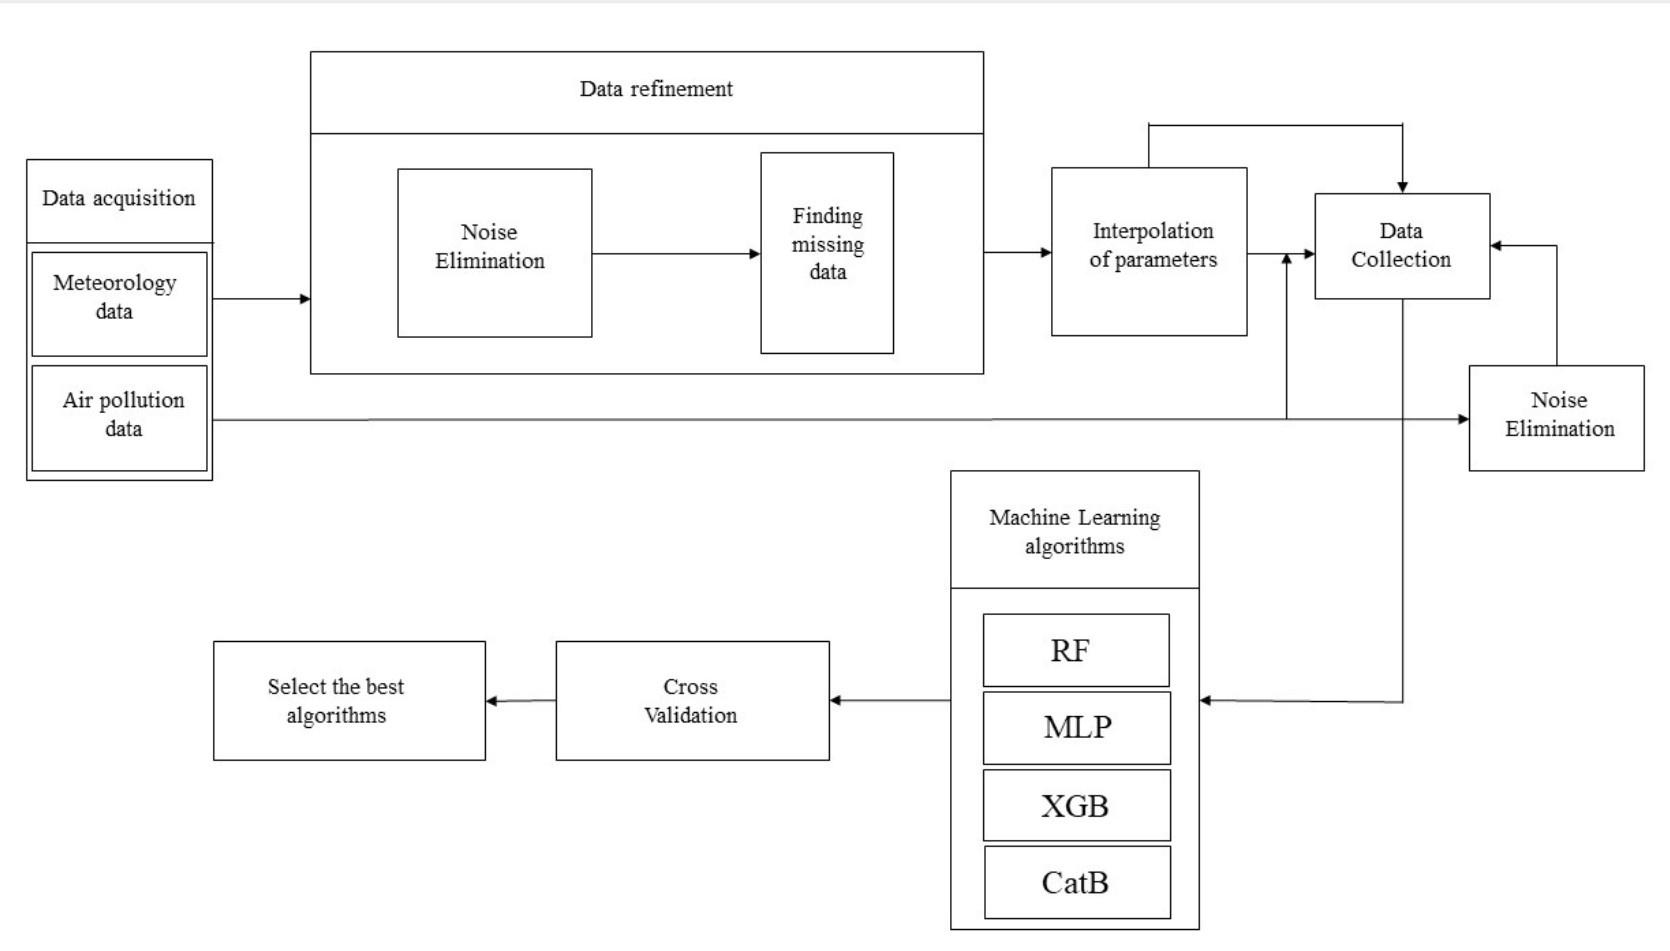
\includegraphics[width= 14 cm]{prearch.jpg}
\caption{Prediction model }
\end{figure}
\pagebreak
The data, which is a combination of both meteorological features and gaseous pollutants is randomly divided into two : Training set and Test set. Usually,it is divided as 70\% for training and 30\% for  test set. Learn models using training set and test the model with test set,from that we select the most accurate model. During training process,the training set is trained using three machine learning algorithms.The algorithms used are : Random Forest, XGBoost, Deep Learning.



\section {Forecast Model}

\begin{figure}[h!]
\label{bc}
\centering
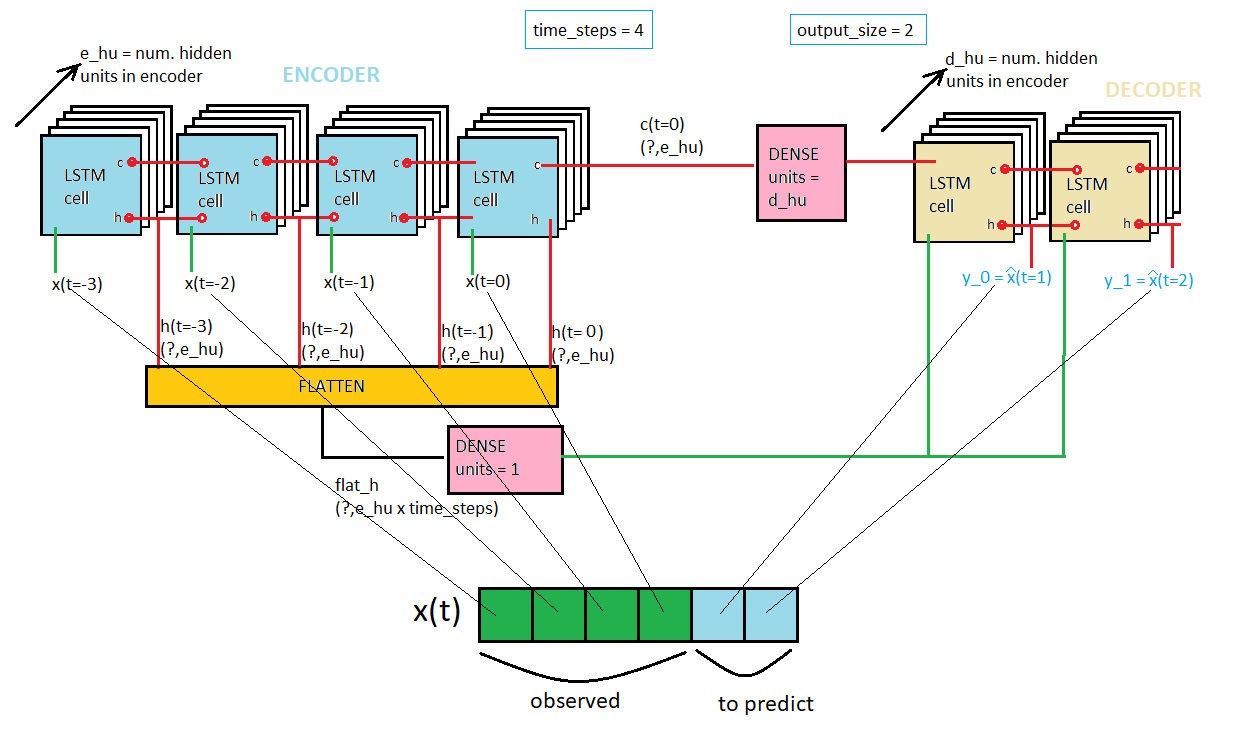
\includegraphics[width= 14 cm]{lstm.png}
\caption{Architecture of the lstm}
\end{figure}


Time series forecasting (TSF) is the task of predicting future values of a given sequence using historical data. Recently, this task has attracted the attention of researchers in the area of machine learning to address the limitations of traditional forecasting methods, which are time-consuming and full of complexity. With the increasing availability of extensive amounts of historical data along with the need of performing accurate production forecasting, particularly a powerful forecasting technique infers the stochastic dependency between past and future values is highly needed. In this paper, we propose a deep learning approach capable to address the limitations of traditional forecasting approaches and show accurate predictions. The proposed approach is a deep long-short term memory (DLSTM) architecture, as an extension of the traditional recurrent neural network. 


\chapter{METHODOLOGIES}  % Short of the project name

\section {Data Pre-processing}
Data pre-processing is a process of cleaning the raw data i.e. the data is collected in the real world and is converted to a clean data set. In other words, whenever the data is gathered from different sources it is collected in a raw format and this data isn't feasible for the analysis.Therefore, certain steps are executed to convert the data into a small clean data set, this part of the process is called as data pre-processing.\par
Data processing and matching is necessary
because the data was obtained from different
sources. Daily climatic data was downloaded
from the IMO portal. There are a few missing
values or in some cases, full day missing records.
Therefore, we used imputation by predictive
mean matching to estimate and fill in the missing
data. The time format of the data was not in good
format and thus was converted to be compatible
with the other data. Missing values for short or
long periods are a common problem in air
pollution monitoring stations. This happens when
there is a critical failure or temporary power
cutoff. There are many missing values that cannot
be compensated by interpolation.
\pagebreak
\subsection{Data Distribution}
\begin{figure}[h!]
\label{bc}
\centering
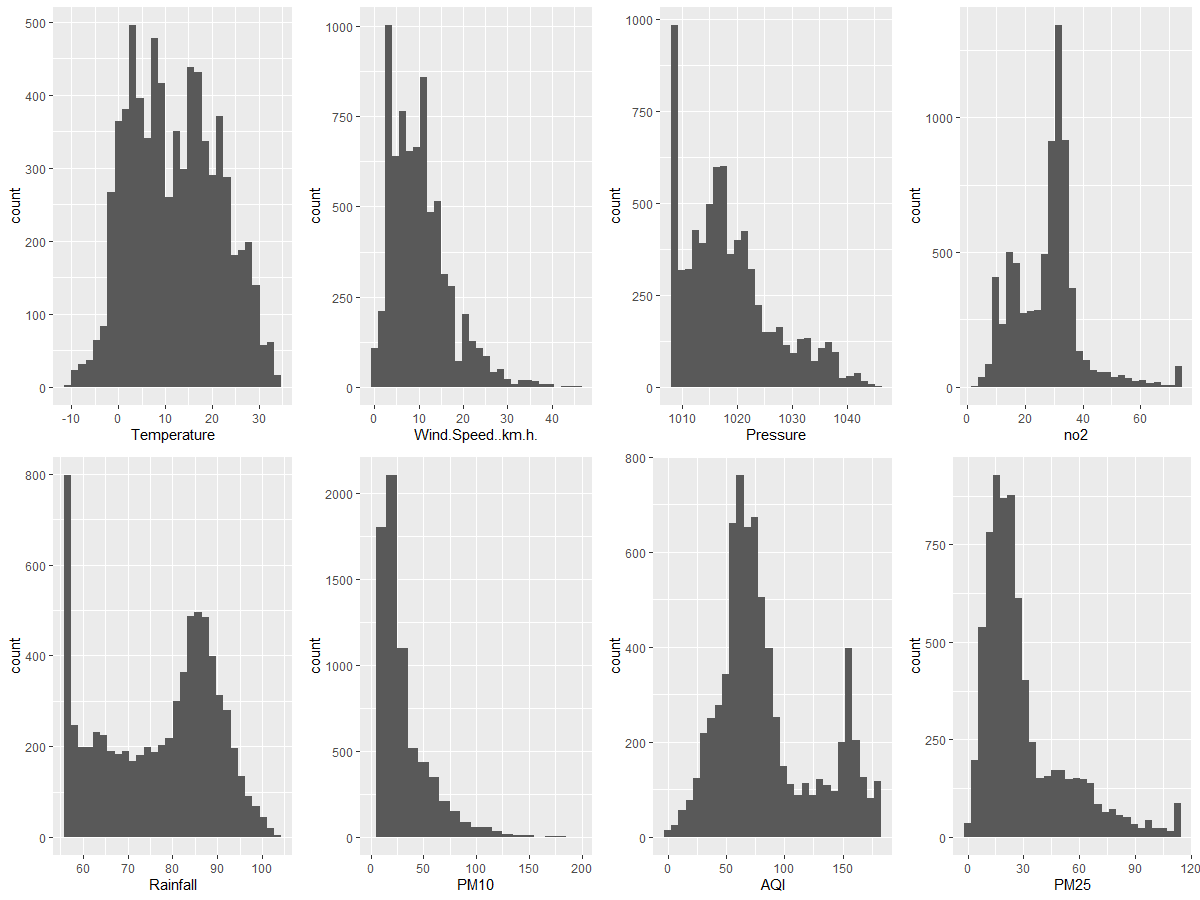
\includegraphics[width= 16 cm]{Histogram.png}
\caption{Static Analysis}
\end{figure}
Outliers are extreme values that deviate from other observations on data , they may indicate a variability in a measurement, experimental errors or a novelty. In other words, an outlier is an observation that diverges from an overall pattern on a sample.we can find outliers by checking histograms or densiity plot of the data.

\subsection{Correlation}
Correlation is a measure of how strongly one variable depends on another.Correlation is
a bivariate analysis that measures the strength of association between two variables and
the direction of the relationship. In terms of the strength of relationship, the value of the
correlation coefficient varies between +1 and -1. A value of +1 or -1 indicates a perfect
degree of association between the two variables.
\subsubsection{Spearman rank correlation}
Spearman rank correlation is a non-parametric test that is used to measure the degree of
association between two variables. The Spearman rank correlation test does not carry any
assumptions about the distribution of the data and is the appropriate correlation analysis
when the variables are measured on a scale that is at least ordinal.The assumptions of the Spearman correlation are that data must be at least ordinal
and the scores on one variable must be monotonically related to the other variable
\begin{figure}[h!]
\label{bc}
\centering
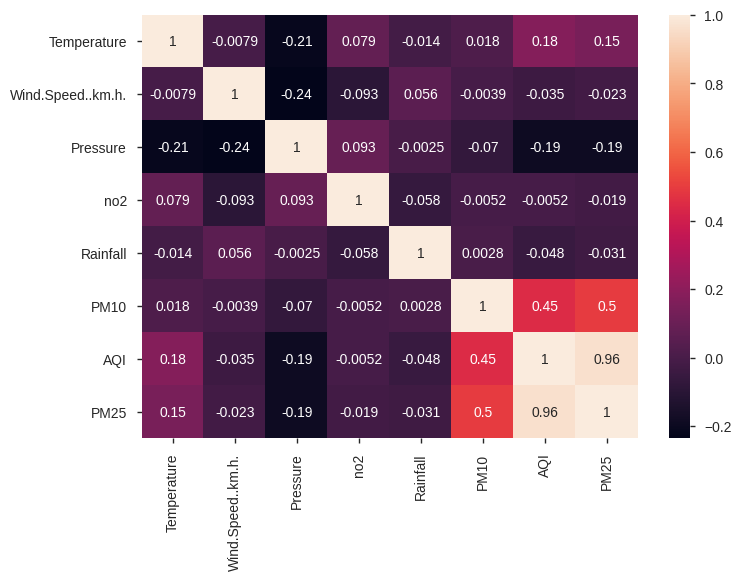
\includegraphics[width= 14 cm]{corr.png}
\caption { Correlation}
\end{figure}
\subsection{Normalization}
Normalization is a technique often applied as part of data preparation for machine learning. The goal of normalization is to change the values of numeric columns in the dataset
to a common scale, without distorting differences in the ranges of values. For machine
learning, every dataset does not require normalization. It is required only when features
have different ranges.Data normalization is an important step for many machine-learning
estimators, particularly when dealing with deep learning. The preferred range of features
for most ML approaches is between -1 to 1. Features with a wider range can cause instability during the model training Standardization was used to standardize the features
by deducting the mean and scaling the data, with the variance of feature. After applying standard normalizations,train and test datasets were prepared. Dataset records were
shuffled and split to 70\% for the train and 30\% for the test.
\subsubsection{Z-Score}
Z-score normalization is also known as zero-mean normalization. Z-score normalization
technique normalizes the input values in the dataset using mean and standard deviation.
The mean and standard deviation for each feature vector is calculated across the training dataset. This normalization technique determines whether an input value is below
or above the average value. It will be very useful to normalize the dataset when the
attribute’s maximum or minimum values are unknown and outliers dominate the input
values.	
\subsection{Imputation}
Imputation is a term replace the missing values by some predictable which said to be
plausible values in the dataset. It makes use of observed supporting information for cases
with non-response maintain high accuracy.
\subsubsection{Prediction mean matching Imputation}
Predictive mean matching imputation is hot deck imputation within classes where the
classes are defined based on the range of the predicted values from the imputation model.
This method achieves a more even spread of donor values for imputation within classes,
which reduces the variance of the imputed estimator. Donor values within classes may
be drawn with or without replacement, where without replacement is expected to lead to
a further reduction in the variance.
\section{Air Quality Prediction}
\subsection{Random Forest Modeling}
Random forests are a combination of tree predictors
such that each tree depends on the values of a random
vector sampled independently and with the same
distribution for all trees in the forest. The
generalization error for forests converges a.s. to a limit
as the number of trees in the forest becomes large.
The generalization error of a forest of tree classifiers
depends on the strength of the individual trees in the
forest and the correlation between them. 
\par
Random Forests are trained via the bagging method. Bagging or Bootstrap Aggregating, consists of randomly sampling subsets of the training data, fitting a model to these smaller data sets, and aggregating the predictions. This method allows several instances to be used repeatedly for the training stage given that we are sampling with replacement. Tree bagging consists of sampling subsets of the training set, fitting a Decision Tree to each, and aggregating their result.
In the Random Forests algorithm, each new data point goes through the same process, it visits all the different trees in the ensemble, which are were grown using random samples of both training data and features. Depending on the task at hand, the functions used for aggregation will differ. For Classification problems, it uses the mode or most frequent class predicted by the individual trees, whereas for Regression tasks, it uses the average prediction of each tree.
\begin{figure}[h]
\label{ss}
\centering
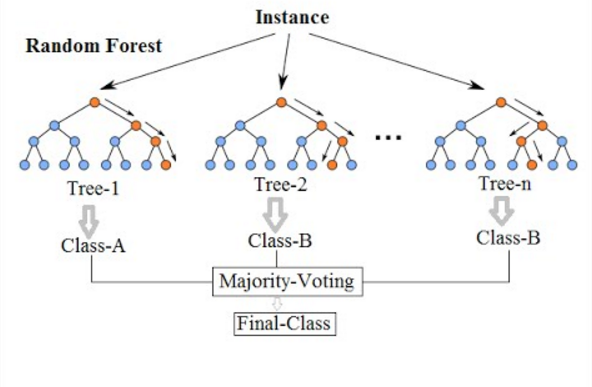
\includegraphics[width= 10 cm]{rf.png}
\caption{Random Forest}
\end{figure}
\subsubsection{Procedure}
Random forest is a supervised ensembling
learning method, introduced by Ho [6], that acts
based on decision trees. it is very flexible
and fast. To conduct RF analysis, it is necessary
to adjust a model’s hyperparameters. A grid
search for model performance optimization was
carried out with the 10-fold cross-validation
technique based on the R square metric.
\begin{figure}[h]
\label{ss}
\centering
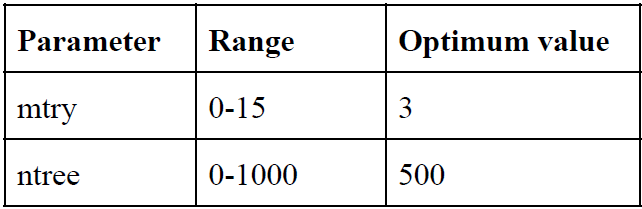
\includegraphics[width= 10 cm]{rftable.png}
\caption{Table: Random Forest Parameters}
\end{figure}

\subsubsection{K-fold Cross Validation}
The objective is to choose different partitions of training set and validation set, and then average the result, so that the result will not be biased by any single partition.In k-fold cross-validation, the original sample is randomly partitioned into k equal sized subsamples. Of the k subsamples, a single subsample is retained as the validation data for testing the model, and the remaining subsamples are used as training data. The cross-validation process is then repeated k times, with each of the k subsamples used exactly once as the validation data. The k results can then be averaged to produce a single estimation. The advantage of this method over repeated random sub-sampling is that all observations are used for both training and validation, and each observation is used for validation exactly once. 10-fold cross-validation is commonly used, but in general k remains an unfixed parameter.
The ntree parameter specifies the number of trees to grow. In the random forests literature, this is referred to as the ntree parameter. Larger number of trees produce more stable models and covariate importance estimates, but require more memory and a longer run time. For small datasets, 50 trees may be sufficient. For larger datasets, 500 or more may be required.
The mtry parameter specifies the number of variables available for splitting at each tree node. In the random forests literature, this is referred to as the mtry parameter. The default value of this parameter depends on which R package is used to fit the model:

RandomForest - For classification models, the default is the square root of the number of predictor variables (rounded down). For regression models, it is the number of predictor variables divided by 3 (rounded down).

Party - The default is always 5.

There is extensive discussion in the literature about the influence of mtry. Cutler et al. (2007) reported that different values of mtry did not affect the correct classification rates of their model and that other performance metrics (sensitivity, specificity, kappa, and ROC AUC) were stable under different values of mtry. On the other hand, Strobl et al. (2008) reported that mtry had a strong influence on predictor variable importance estimates.
We make use of grid search to tune the parameters mtry and ntree, for obtaining accurate predictions from our model.


\subsubsection{Accuracy}
Accuracy is a nice metric for classification, but it doesn’t really make sense in the context of regression. Instead, we will use root mean square error (RMSE) to estimate how well our random forest was able to predict our test set outcomes. RMSE or Root Mean Squared Error is the average deviation of the predictions from the observations. It is useful to get a gross idea of how well (or not) an algorithm is doing, in the units of the output variable.
\begin{figure}[h]
\label{ss}
\centering
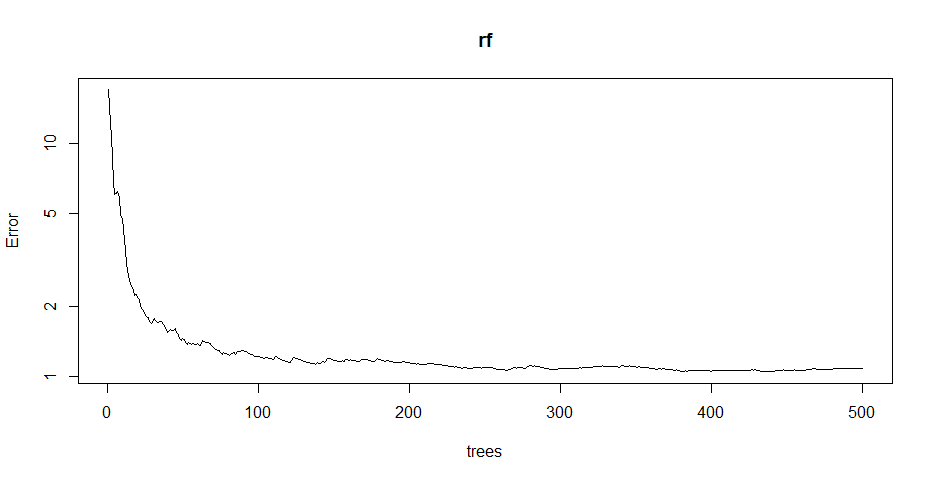
\includegraphics[width= 10 cm]{rf_nooftrees_vs_error.png}
\caption{Plot of number of trees vs Error}
\end{figure}
\pagebreak

The variables importance measures can be plotted using the function varImpPlot(),as shown in the fisgure below:
\begin{figure}[h]
\label{ss}
\centering
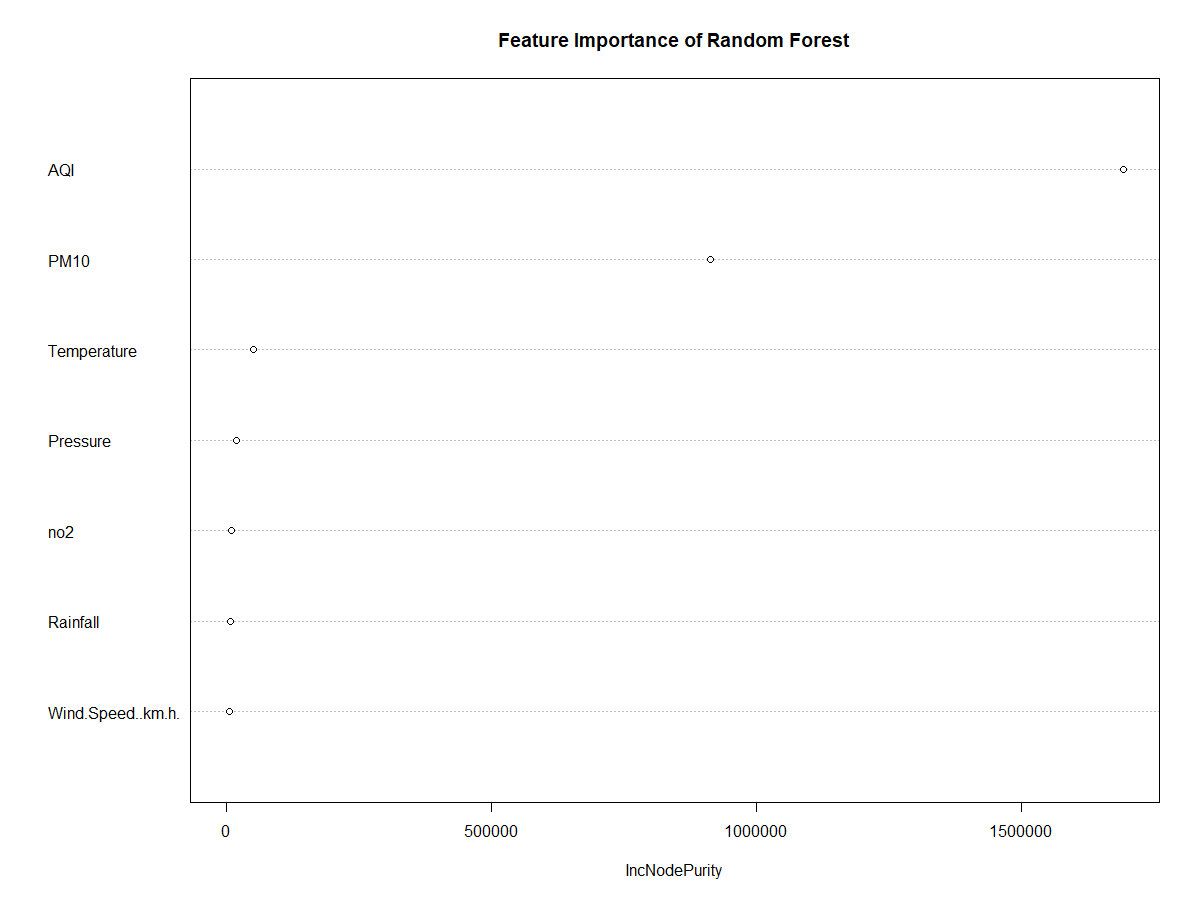
\includegraphics[width= 10 cm]{rf_freature_importence.png}
\caption{Feature Impotance}
\end{figure} 
\linebreak
A histogram representation to show the frequency of the trees with particular number of nodes in our random forest model:\linebreak
\begin{figure}[h]
\label{ss}
\centering
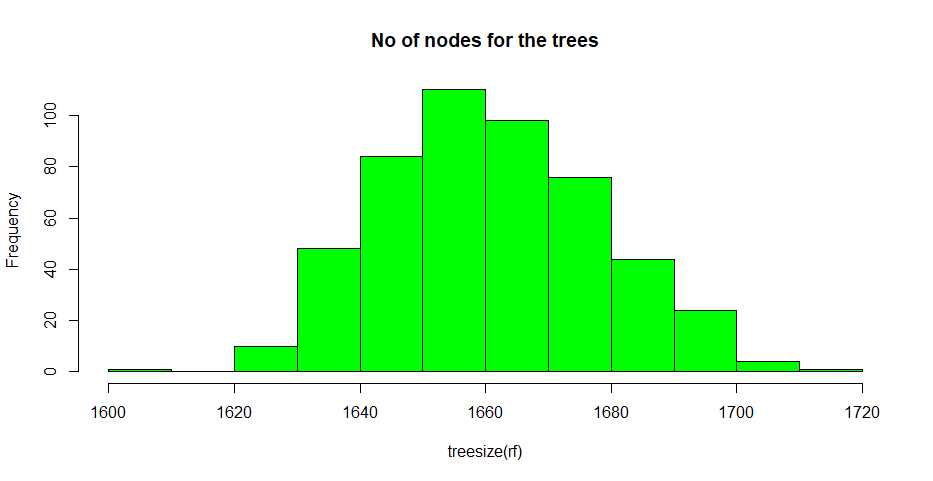
\includegraphics[width= 11 cm]{rf_no_of_nodes_for_the_trees.png}
\caption{Histogram}
\end{figure}\pagebreak

\subsection{Deep Learning}
Deep learning is one of the machine learning methods that is based on its ancestor—the Artificial Neural Network (ANN).
The most beautiful thing about Deep Learning is that it is based upon how we, humans, learn and process information. Everything we do, every memory we have, every action we take is controlled by our nervous system which is composed of neurons! The simplest of the ANNs can be created from three layers of “neurons”. The input layer, the hidden layer and the output layer. Information flows from the input layer, through the hidden layer to the output layer and then out.\linebreak
\begin{figure}[h]
\label{ss}
\centering
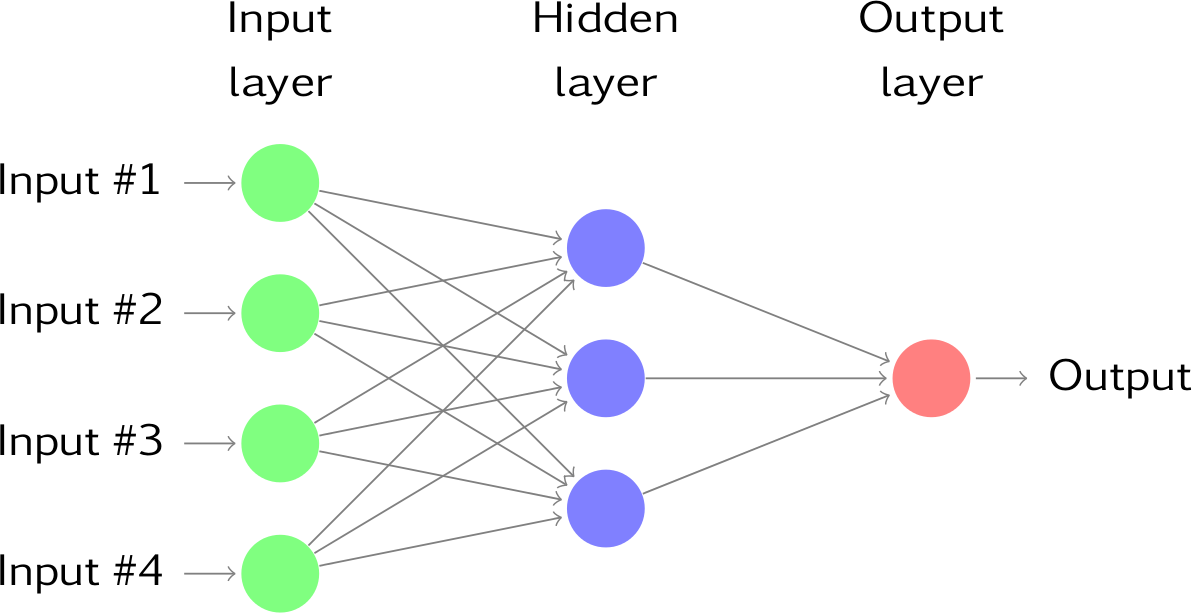
\includegraphics[width= 14 cm]{deep.png}
\caption{Simple Artificial Neural Network}
\end{figure} \linebreak

When a neural network is being trained. it is provided with a set of inputs as well as their corresponding outputs. It runs the inputs through the neurons on each of the layers of the network, and using the parameters above, each neuron transforms the input in some way and forwards it to the next layer and so on. The result that it receives on the output layer is then compared to the outputs supplied above and it checks how far apart the two are and accordingly adjusts the parameters on each of the neurons through special algorithmsdesigned to bring the actual and produced outputs as close to each other as possible. It learns to adjust its weights and threshold values to arrive at the correct output. This is what we call as “learning” for the artificial neural network. This process is repeated a (very high) number of times until the produced and expected outputs are as close as possible. That completes the training.when new inputs are supplied to the neural network, we can confidently say that the predicted outputs of the network will be fairly close to the actual outputs. Such ANNs can be used in predicting based upon certain features and classifying objects and images.\\
Such neural networks which consist of more than three layers of neurons (including the input and output layer) are called as Deep Neural Networks. And training them is called as Deep Learning. \linebreak

\subsubsection{Multilayer Perceptron}
A multilayer perceptron (MLP) is a class of
feedforward artificial neural network (ANN). To
measure the performance of the regressor the loss
function is defined Sometimes the problem of
overfitting and underfitting occurs at the time of
training the model. In order to train the network,
an optimization procedure is required for this. We
need loss function and an optimizer. This
procedure will find the values for the set of
weights, W that minimizes the loss function.

\begin{figure}[h]
\label{ss}
\centering
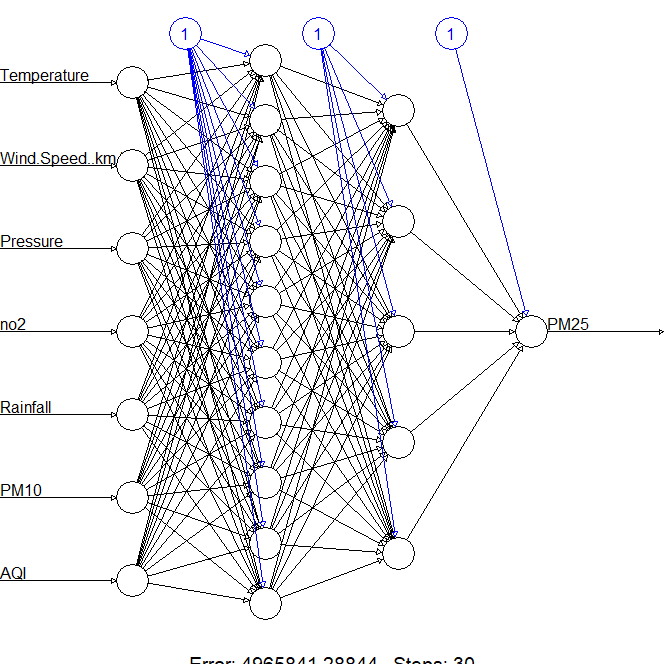
\includegraphics[width= 11 cm]{deep_nue_mod.png}
\caption{Neural Network Model}
\end{figure} \pagebreak

\par
Procedure:
AQI is set as the dependent variable,and the rest of the  features are set as the independent variables.The data is converted into a matrix form,and is split into two independent samples, training and testing, 70 percent and 30 percent respectively.The test and train samples are then normalised, using Z Normalization.The tuned model has two hidden layer, with ten and five neurons. The activation function used in Rectified Linear Unit (relu). The input layer has one neuron each for the independent variables,and the output layer has one neuron for response. As we are using regression and the output variable is numeric, mse  is used as the loss function ,and rmsprop is used as the optimizer function and mae is used as the metric function , to compile the model.To fit the model,the training data is used ,which is run over a 100 epochs,then to evaluate the model ,the testing data is used. The test data is used for getting the prediction.
\begin{figure}[h]
\label{ss}
\centering
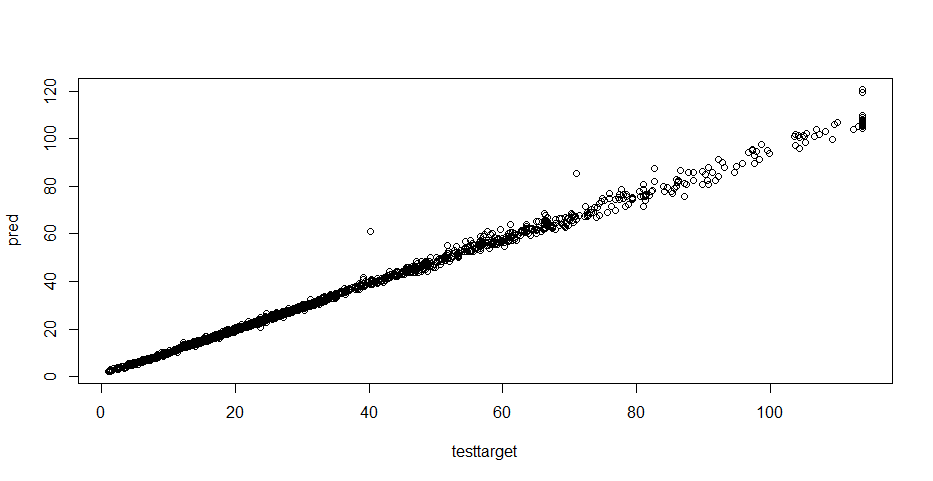
\includegraphics[width= 14 cm]{deep_target_vs_prediction_plot.png}
\caption{Predicted vs Testtarget Plot}
\end{figure}\pagebreak

\subsection{XGBoost modelling}
XGBoost is an ensemble learning algorithm that follows the principle of boosting. Boosting is a general term in ML where multiple weak learners such as regression trees are ensembled to create a single strong learner. The basic idea behind this procedure is to learn sequentially in which the current regression tree is fitted to the residuals (errors) from the previous trees. This new regression tree is then added to the fitted model to update the residuals. It is worth noting that statistical learning approaches that learn slowly such as boosting tend to perform well . The principle of gradient boosting further enhances the flexibility of the boosting algorithm by constructing the new regression trees to be maximally correlated to the negative of the gradient of the loss function. 
XGBoost is based on a gradient boosting algorithm proposed by Tianqi Chen .The XGBoost similar to the random forest is tuned using hyperparameters. A grid search on hyperparameters with 10-fold cross-validation was carried out to find the best model based on R square metrics.\linebreak

\begin{figure}[h]
\label{bd}
\centering
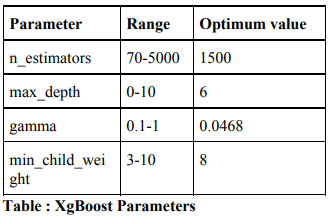
\includegraphics[width= 11 cm]{xg1.png}
\caption{Parameters}
\end{figure}
The root mean square value of xgboost is obtained as 0.7457792.\pagebreak

\subsubsection{Cross validation in xgboost}
Cross validation is a statistical method to evaluate machine learning models on unseen data. It comes in handy when the dataset is limited and prevents overfitting by not taking an independent sample (holdout) from training data for validation. By reducing the size of training data, we are compromising with the features and patterns hidden in the data which can further induce errors in our model. This is similar to cross\_val\_score functionality provided by the caret library. XGBoost uses built-in cross validation function cv():
xgb.cv()\par
2. k-fold Cross-validation — In k-fold cross-validation, data is shuffled and divided into k equal sized subsamples. One of the k subsamples is used as a test/validation set and remaining (k -1) subsamples are put together to be used as training data. Then we fit a model using training data and evaluate using the test set. This process is repeated k times so that every data point stays in validation set exactly once. The k results from each model should be averaged to get the final estimation. The advantage of this method is that we significantly reduce bias and variance and also increase the robustness of the model. 
\begin{figure}[h]
\label{bd}
\centering
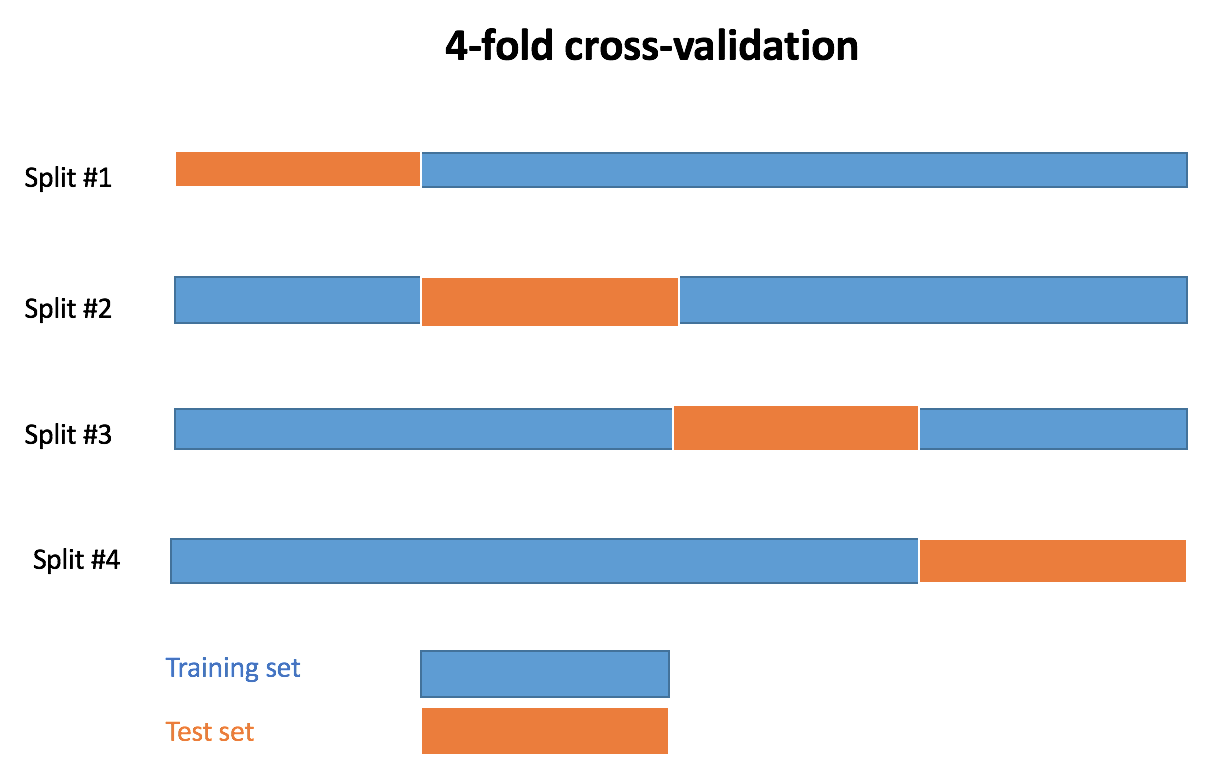
\includegraphics[width= 14 cm]{xgb_kfold.png}
\caption{cross-validation}
\end{figure}
\subsubsection{Feature Importance}
Although it is important to be proficient in
understanding the inner workings of the
algorithm, Just showing that the algorithm
predicts well is not enough. You have to attribute
the predictions to the elements of the input data
that contribute to your accuracy. feature
importances which helps us explain the predictive
power of the features in the dataset.\par
\begin{figure}[h]
\label{bd}
\centering
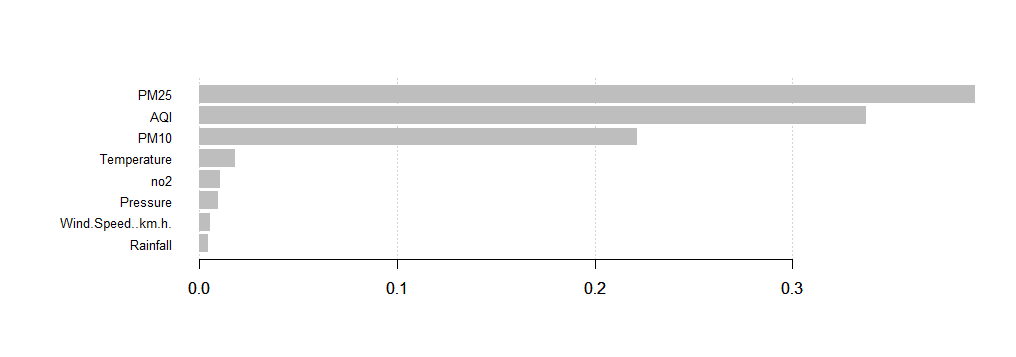
\includegraphics[width= 15 cm]{xgbimp.png}
\caption{Feature Importance of xgBoost}
\end{figure}

\subsection{CatBoost modelling}
CatBoost is a new gradient boosting decision tree (GBDT) algorithm that can handle categorical features well. “CatBoost” name comes from two words “Category” and “Boosting”. This algorithm is different from traditional GBDT algorithms. One main difference between CatBoost and other boosting algorithms is that the CatBoost implements symmetric trees.
   CatBoost is an ensemble of symmetric decision trees, whose symmetry structure endows it fewer parameters, faster training and testing, and higher accuracy. In addition, CatBoost replaces the gradient estimation method of the traditional gradient boosting algorithm with ordered boosting, thereby reducing the bias of the gradient estimation and improving the generalization capability
The root mean square value of catboost is obtained as 0.6030147.

\begin{figure}[h]
\label{bd}
\centering
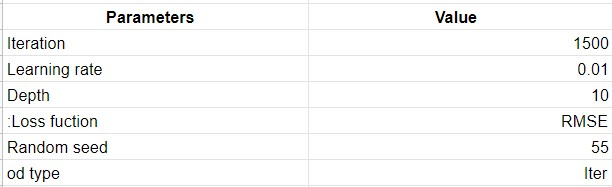
\includegraphics[width= 7 cm]{cat1.jpg}
\caption{Parameters}
\end{figure}

 \subsubsection{Feature Importance}
 Sometimes it
is just as important to understand how the features
in our model contribute to prediction. The feature
importances from xgboost are	
calculated based on the training data given to the
model, not on predictions on a test dataset.by
getting a better understanding of the model’s
logic you can not only verify it being correct but
also work on improving the model by focusing
only on the important variables
\begin{figure}[h]
\label{bd}
\centering
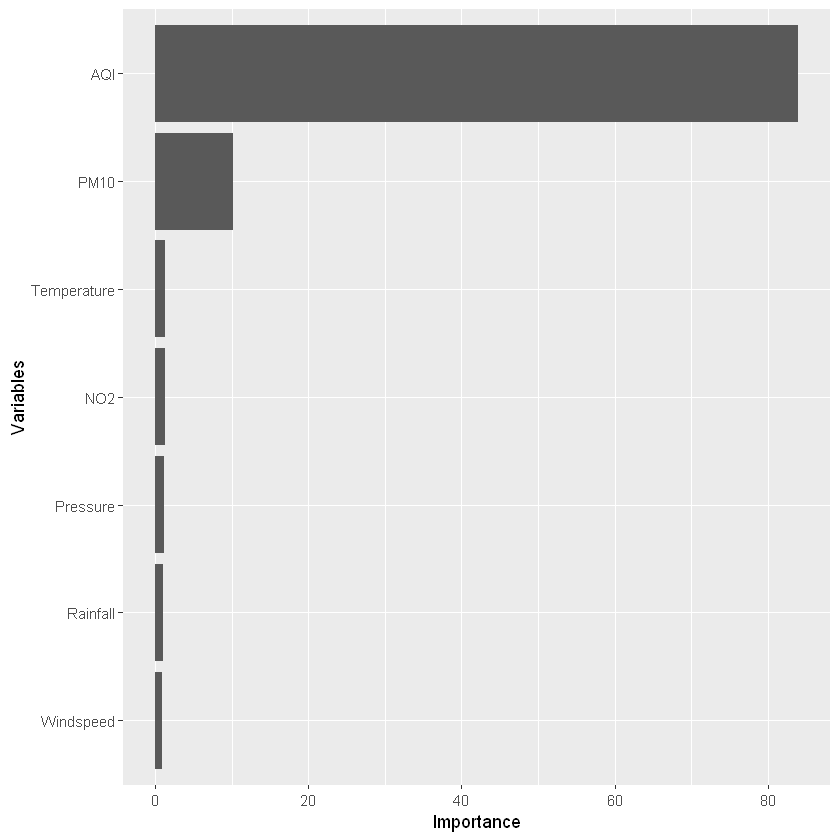
\includegraphics[width= 8 cm]{catimp.png}
\caption{Feature Importance of catBoost}
\end{figure}
\pagebreak
\section{Air Quality Forecast}

\subsection{Prophet}
Prophet is applied on the time series data set to
forecast the PM2.5 value 7 days prior to the
current date, producing the RMSE to be 24.00.
This is achieved by using historical data of PM2.5
for the last 5 years.
Prophet is a open source package for forecasting that is introduced by facebook. It is also used for finding the trend, weekly and yearly seasonality in the time series data.
Prophet is a procedure for forecasting time series
data based on an additive model where non-linear
trends are fit with yearly, weekly, and daily
seasonality, plus holiday effects. It works best
with time series that have strong seasonal effects
and several seasons of historical dataProphet is a procedure for forecasting time series
data based on an additive model where non-linear
trends are fit with yearly, weekly, and daily
seasonality, plus holiday effects. It works best
with time series that have strong seasonal effects
and several seasons of historical data

\begin{figure}[h]
\label{bd}
\centering
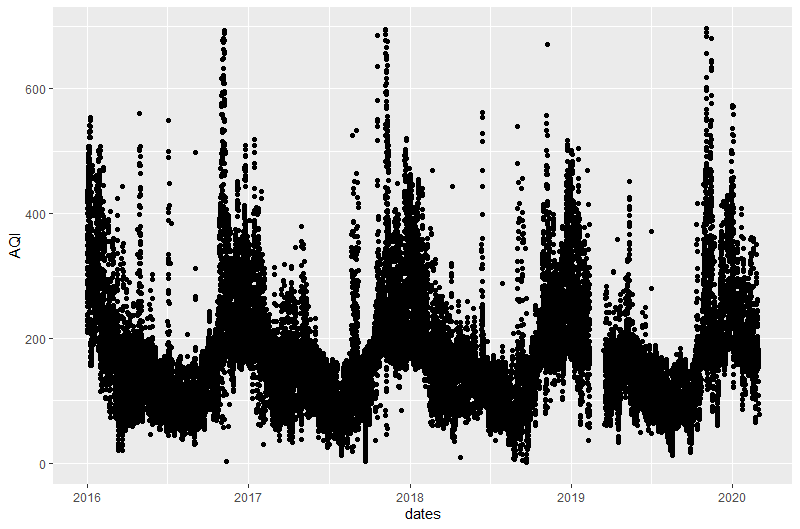
\includegraphics[width= 15 cm]{proph1.png}
\caption{Forecast}
\end{figure} \pagebreak

\begin{figure}[h]
\label{bd}
\centering
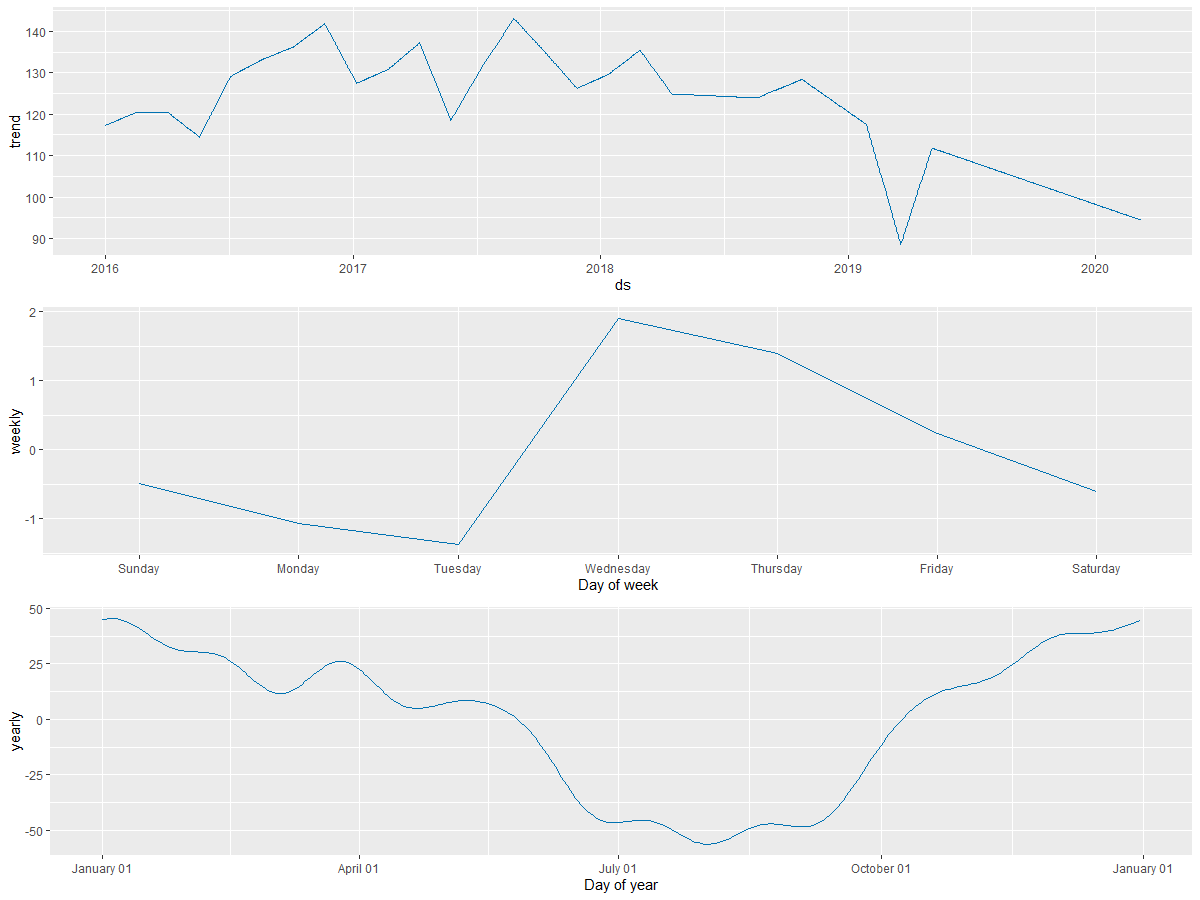
\includegraphics[width= 11 cm]{r1.png}
\caption{Yearly weekly seasonality and trend}
\end{figure}

\subsection{Long Short-Term Memory networks(LSTM)}

We are using a Univariate LSTM model from many univariate LSTM we select CNN LSTM model.
The CNN can be very effective at automatically extracting and learning features from univarient data. Model can be used in a hybrid model with an LSTM backend where the CNN is used to interpret subsequences of input that together are provided as a sequence to an LSTM model to interpret
\begin{figure}[h]
\label{bd}
\centering
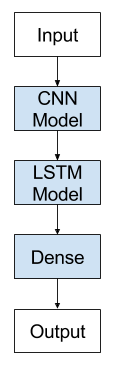
\includegraphics[width= 2.2 cm]{lstm_org.png}
\caption{Working of CNN LSTM}
\end{figure}

\subsubsection{Parameters}

\begin{figure}[h]
\label{bd}
\centering
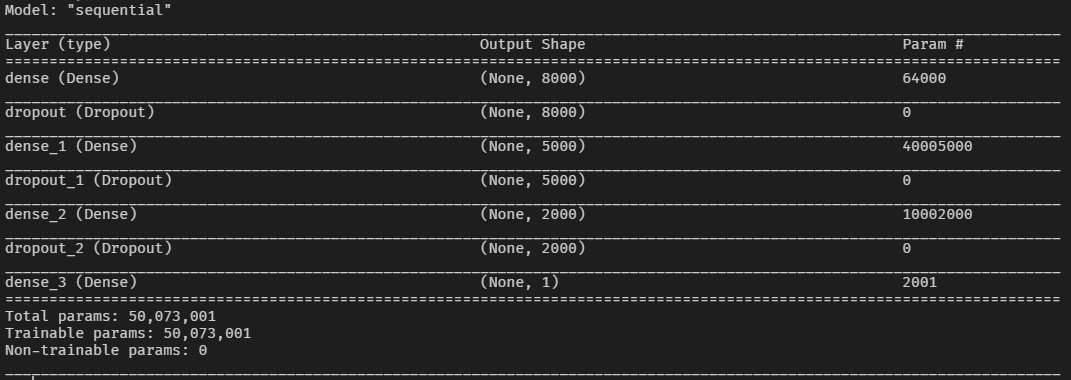
\includegraphics[width= 15 cm]{lstm_para.jpg}
\caption{Summary of the model}
\end{figure}
\begin{figure}[h]
\label{bd}
\centering
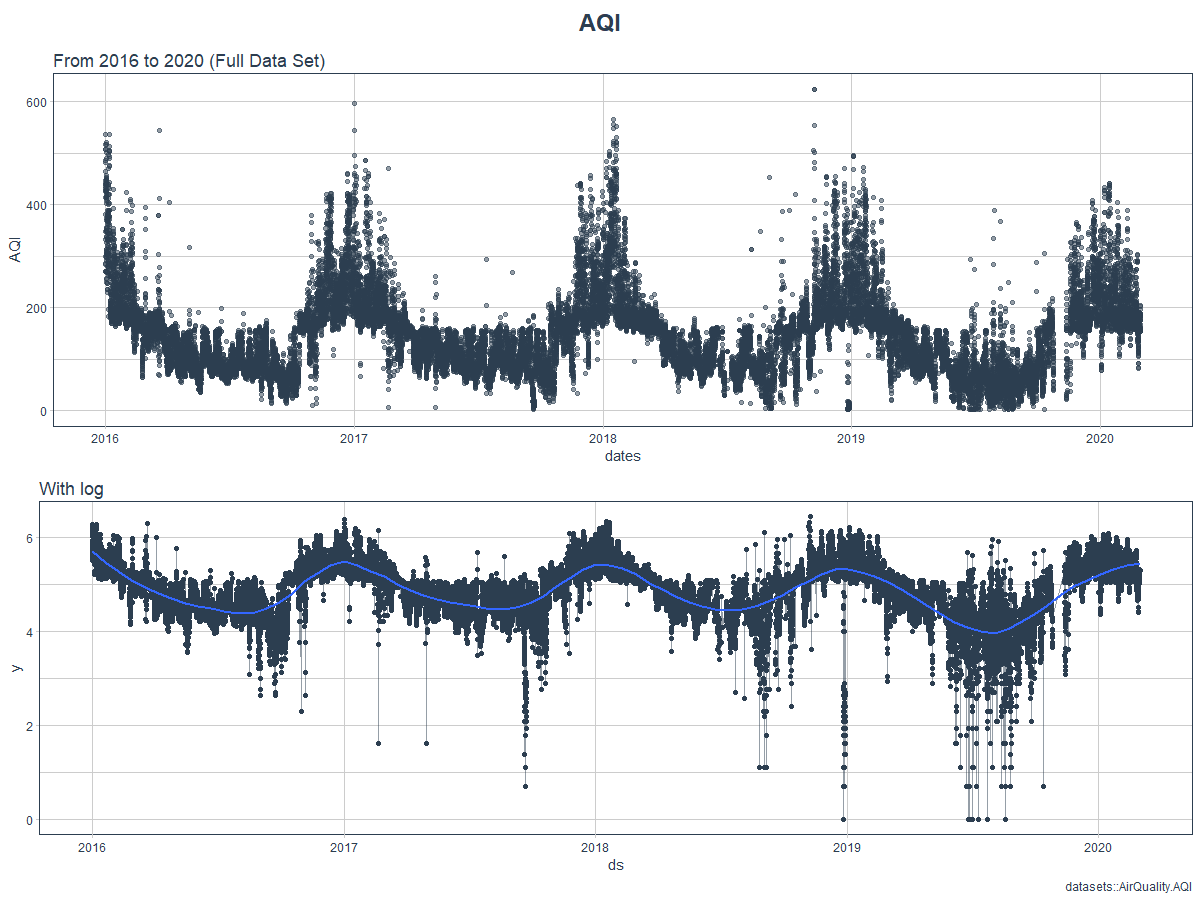
\includegraphics[width= 14 cm]{proph.png}
\caption{model plot}
\end{figure}

 This model is producing the RMSE of 18.64

\chapter{IMPLEMENTATION AND  DEPLOYMENT}
\section{Software Requirements}
These are main sofware requirements to implement the proposed solution
\subsection{Rstudio}
a free open source integrated development enviornment for R. Rstudio helps keeps R more organized and it adds more functionality to it. R is maily used for statistical and quantitative analysis R provides a wide variety of statistical
and graphical techniques, and is highly extensible.One of R’s strengths is the ease with which well-designed publication-quality plots can be produced, including mathematical symbols and formulae where needed. Great care has been taken over the defaults for the minor design choices in graphics, but the user retains full control.

\subsection{Shiny}
Shiny is an open source R package that provides an elegant and powerful web framework for building web applications using R. Shiny helps you turn your analyses into interactive web applications without requiring HTML, CSS, or JavaScript knowledge.\pagebreak

\subsection{Tensorflow}
ensorFlow is an open-source software library released in 2015 by Google to make it
easier for developers to design, build, and train deep learning models. TensorFlow is
available on different operating systems such as Linux, Windows, macOS, and also on
mobile operating platforms like iOS and Android. One of the salient features of Tensorflow  is that it is capable of running on multiple CPUs and GPUs. The computations
in Tensor-Flow are reported as stateful dataflow graphs. TensorFlow is considered the
first serious implementation of a framework focused on deep learning. TensorFlow can
trainandrundeepneuralnetworksforhandwrittendigitclassification, imagerecognition,
word embeddings, recurrent neural networks, sequence-to-sequence models for machine
translation, natural language processing, and PDE (partial differential equation) based
simulations. TensorFlow supports production prediction at scale, with the same models
used for training.

\subsection{Keras}

Keras is a high-level neural networks API, written in Python and capable of running on
top of TensorFlow, CNTK, or Theano. It was developed with a focus on enabling fast
experimentation. It focuses on being user-friendly, modular, and extensible. It was devel-
oped as part of the research effort of project ONEIROS (Open-ended Neuro-Electronic
Intelligent Robot Operating System). Keras contains numerous implementations of com-
monly used neural-network building blocks such as layers, objectives, activation func-
tions, optimizers, and a host of tools to make working with image and text data easier.
In addition to standard neural networks, Keras has support for convolutional and re-
current neural networks. It supports other common utility layers like dropout, batchnor-
malization, and pooling.
Keras allows users to productize deep models on smartphones (iOS and Android),
on the web, or on the Java Virtual Machine. It also allows use of distributed training
of deep-learning models on clusters of Graphics Processing Units (GPU) and Tensor
processingunits (TPU).

\section{Implementation}
We developed  4 models for air quality prediction and 2 models for air quality forecasting.
All the predictive model is trained using the dataset and save all the model in rds format 
All the forecasting model is trained using 5 years of historical data of air quality index.
for LSTM model is saved in the tensorflow savedmodel format
and prophet model saved in rds format.
\section{Deployment}
   Our team developed the model in RStudio using R programming. RStudio Shiny is an excellent tool for building and deploying models. Shiny provides the ability to build reactive web applications all in R programming language. 
    We deployed our prediction model using Shiny. There are several tools to help you host a Shiny app, and the most common ones are RStudio Connect, shinyapps.io, and MatrixDS.
In shiny there are many features added like Statistical Summary, Histogram ploting, Finding correlation

\chapter{EVALUATION AND RESULT}

\subsection{Evaluation of Models}

\begin{figure}[h]
\label{bd}
\centering
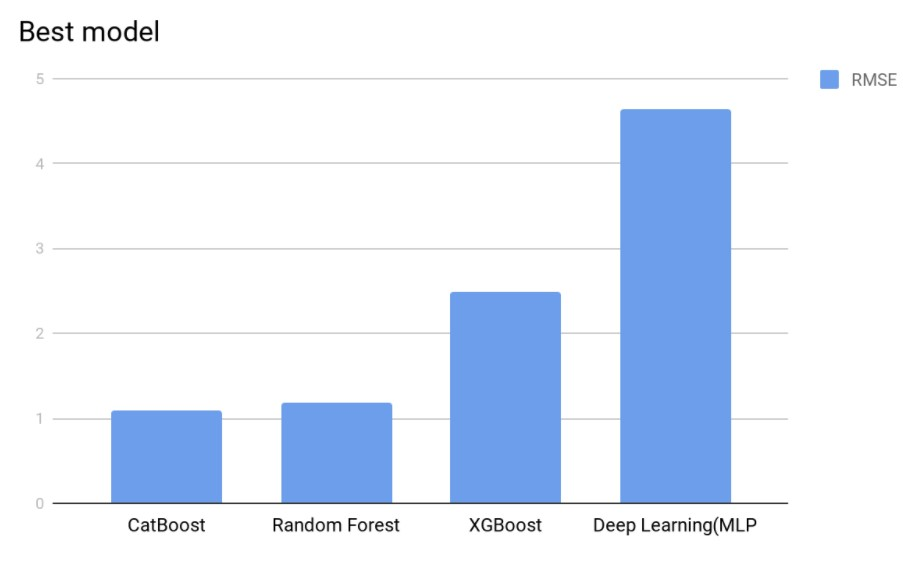
\includegraphics[width= 14 cm]{best_model.jpg}
\caption{model plot}
\end{figure}
We can see that CatBoost and Random forest are the best models with Least error. We can use this model in any web app or mobile app.
to predict the amount of PM 2.5. In Prophet forecsting RMSE value is 64 AQI and the LSTM model the RMSE Ranges from 80 to 124 AQI.


%%%%%%%%%%%%%%%%%%%%%%%%%%%%%%%%%%%%
%%%%%%%%%%%%%%%%%%%%%%%%%%%%%%%%%%%%
%%
%%          Bibliography 
%%
%%%%%%%%%%%%%%%%%%%%%%%%%%%%%%%%%%%%
%%%%%%%%%%%%%%%%%%%%%%%%%%%%%%%%%%%%

\clearpage
\addcontentsline{toc}{chapter}{\quad BIBLIOGRAPHY}
\begin{thebibliography}{99}
%%%%%%%%%%%%%%%%%%%%%%%%%%%%%%%%%%%%
%%
%%          Add Bibliography from below, here 3 eg are there
%%	    If u need to add more bib  use \bibitem   command again & again
%%
%%%%%%%%%%%%%%%%%%%%%%%%%%%%%%%%%%%%

\bibitem{a}
Xiao Feng, Qi Li, Yajie Zhu, Junxiong Hou, Lingyan Jin, Jingjie Wang,"Artificial neural networks forecasting of PM2.5 pollution using air mass
trajectory based geographic model and wavelet transformation" {\em 1352-2310/ 2015 The Authors. Published by Elsevier Ltd. This is an open access article under the CC BY license}, 


\bibitem{b}
Pandey, Gaurav, Bin Zhang, and Le Jian. \&quot; Predicting sub-micron air pollution indicators: a machine learning approach.\&quot ; Environmental Science: Processes \& amp; Impacts 15.5 (2013): 996-1005.

\bibitem{c}
Dan wei: Predicting air pollution level in a specific city
[2014]

\bibitem{d}
Dixian Zhu, Changjie Cai, Tianbao Yang and Xun Zhou: A
Machine Learning Approach for Air Quality Prediction:
Model Regularization and Optimization. Big data and
cognitive computing [2018].

\bibitem{e}
José Juan Carbajal-Hernándezab Luis P.Sánchez-Fernándeza
Jesús A.Carrasco-OchoabJosé Fco.Martínez-Trinidadb:
Assessment and prediction of air quality using fuzzy logic
and autoregressive models: Center of Computer Research –
National Polytechnic Institute, Av. Juan de Dios Bátiz S/N,
Gustavo A. Madero, Col. Nueva. Industrial Vallejo, 07738
México D.F., Mexico1. (2012) Doi
:https://doi.org/10.1016/j.atmosenv.2012.06.004

\bibitem{f}
Sachit Mahajan, Ling-Jyh Chen, Tzu-Chieh Tsai : An
Empirical Study of PM2.5 Forecasting Using neural network.
IEEE Smart World Congress, At San Francisco, USA [2017]

\bibitem{g}
Xiuwen Yi, Junbo Zhang, Zhaoyuan Wang, Tianrui Li, and Yu Zheng. 2018. Deep
Distributed Fusion Network for AirQuality Prediction. In Proceedings of the 24th
ACM SIGKDD International Conference on Knowledge Discovery \&38; Data Mining (KDD ’18). 965–973.

\bibitem{h}
Rouzbeh Shad, Mohammad Saadi Mesgari, Arefeh Shad, et al. 2009. Predicting
air pollution using fuzzy genetic linear membership kriging in GIS. Computers,
environment and urban systems 33, 6 (2009), 472–481

\bibitem{i}
World Health Organization. WHO Air quality guidelines for particulate matter, ozone, nitrogen dioxide and sulphur dioxide.Global Update
2005.Summary of risk assessment. Google Scholar. 2005.

\bibitem{j}
Songgang Zhao, Xingyuan Yuan, Da Xiao, Jianyuan Zhang, Zhouyuan Li. (2018) "AirNet:a machine learning dataset for air quality
forecasting"

\bibitem{k}
Díaz-Robles L, Ortega J, Fu J, Reed G, Chow J, Watson J, Moncada-Herrera J. (2008) "A hybrid ARIMA and artificial neural networks
model to forecast particulate matter in urban areas: The case of Temuco, Chile." Atmospheric Environment 42: 8331-8340

\bibitem{l}
Liang X, Li S, Zhang S, Huang H, Chen S. (2016) "PM2.5data reliability, consistency, and air quality assessment in five Chinese cities."
Journal of Geophysical Research: Atmospheres 121: 10,220-10,236

\bibitem{m}
Y. Zhang, Y. He, and J. Zhu, ‘‘Research on forecasting problem based
on multiple linear regression model PM2.5,’’ J. Anhui Sci. Technol. Univ.,
vol. 30, no. 3, pp. 92–97, 2016.

\bibitem{n}
K. R. Baker and K. M. Foley, ‘‘A nonlinear regression model estimating
single source concentrations of primary and secondarily formed PM2.5,’’
Atmos. Environ., vol. 45, no. 22, pp. 3758–3767, 2011.

\bibitem{o}
J. B. Ordieresa, E. P. Vergara, R. S. Capuz, and R. E. Salazar, ‘‘Neural
network prediction model for fine particulate matter (PM2.5) on the US–
Mexico border in El Paso (Texas) and Ciudad Juárez (Chihuahua),’’ Envi-
ron. Model. Softw., vol. 20, no. 5, pp. 547–559, 2005.

\bibitem{p}
Bhaskar, B.V., Rajasekhar, R.V.J., Muthusubramaian, P., Kesarkar, A.P., 2008. Measurement and modeling of respirable particulate (PM10) and lead pollution over
Madurai, India. Air Quality, Atmosphere and Health 1, 45e55.
\bibitem{q}
EPA, 1998. National Air Quality and Emissions Trends Report 1997. Environmental
Protection Agency 454:R98e016. Environmental Protection Agency, Oûce of Air
Quality Planning and Standards, Research Triangle Park.
EPA, 1999. Air quality index reporting: final rule. Federal Register. Part III, 40 CFR
Part 58.
\bibitem{r}
Gorunescu, F., 2011. Data Mining Concepts, Models and Techniques, Intelligent
System Reference Library. Springer-Verlag, Heidelberg. http://dx.doi.org/10.
1007/978-3-642-19721-5.
\bibitem{s}
Singh, K.P., Gupta, S., Kumar, A., Shukla, S.P., 2012. Linear and nonlinear modeling
approaches for urban air quality prediction. Science of the Total Environment
426, 244e255.
\bibitem{t}
Swamy, M.N., Hanumanthappa, M., 2012. Predicting academic success from student
enrolment data using decision tree technique. International Journal of Applied
Information Systems 4, 1e6.

\end{thebibliography}



%%%%%%%%%%%%%%%%%%%%%%%%%%%%%%%%%%%%%
%%%%%%%%%%%%%%%%%%%%%%%%%%%%%%%%%%%%%

%%%%%%%%%%%%%%%%%%%%%%%%%%%%%%%%%%%%%
%%                          
%%		APPENDIX
%%    if u have pgms make that a pdf & add it here, like the data sheets
%%
%%    If you need to give an Intro to the Appendix
%%                                 Otherwise Delete it . . . 
%%
%%%%%%%%%%%%%%%%%%%%%%%%%%%%%%%%%%%%%
%%%%%%%%%%%%%%%%%%%%%%%%%%%%%%%%%%%%%

%%%%%%%%%%%%%%%%%%%%%%%%%%%%%%%%%%%%%
%%%%%%%%%%%%%%%%%%%%%%%%%%%%%%%%%%%%%
%%                      
%%                      For Adding PDF (Data Sheets) for the Appendix
%%
%%%%%%%%%%%%%%%%%%%%%%%%%%%%%%%%%%%%%
%%%%%%%%%%%%%%%%%%%%%%%%%%%%%%%%%%%%%

%%%%%%%%%%%%%%%%%%%%%%%%%%%%%%%%%%%%%
%%%%%%%%%%%%%%%%%%%%%%%%%%%%%%%%%%%%%
%%%%%%%%%%%%%%%%%%%%%%%%%%%%%%%%%%%%%
%%%%%%%%%%%%%%%%%%%%%%%%%%%%%%%%%%%%%


%%%%%%%%%%%%%%%%%%%%%%%%%%%%%%%%%%%%%
%%%%%%%%%%%%%%%%%%%%%%%%%%%%%%%%%%%%%
%
%   Hi, All
%   Arun Xavier, VAST Thrissur
%
%   for more  Visit my Page - http://arunxeee.blogspot.in/
%
%%%%%%%%%%%%%%%%%%%%%%%%%%%%%%%%%%%%
%%%%%%%%%%%%%%%%%%%%%%%%%%%%%%%%%%%%

%
\end{spacing}
\newpage
\thispagestyle{empty}
\vspace*{\fill}
\begin{flushright}

\includegraphics[width=2.5 cm]{VidyaLogo.JPG}\\[.2 cm]
{\Large \bf \rm  Department of \vdept\ }\\
{\large \rm Vidya Academy of Science \& Technology\\
Thalakkottukara, Thrissur - 680 501\\
({\tt http://www.vidyaacademy.ac.in})}
\end{flushright}

%
\end{document}



%%%%%%	Any Problems Contact me  @  arunxeee.blogspot.com
%%%%%								      aruncx@gmail.com
%%%%%%%%%%%%%%%%
%%%%
%%%%
%%%%%%%%%%%
%%
%